\section{Datenanalyse}

	Dieser Abschnitt umfasst die Auswertung der aufgenommenen Daten.
	Im Folgenden werden die Unsicherheiten sämtlicher Messdaten, Messwerte und Messergebnisse nach GUM\cite{1} bestimmt.
	Für weitere Angaben wird an dieser Stelle auf den Anhang in \cref{sec:anhang} verwiesen.
	Alle konkreten Fit-Parameter finden sich ebenfalls im Anhang in \cref{sec:anhang}.

\subsection{Verzögerungsdauer}
	
	Um möglichst viele Koinzidenzen zu messen, wird die Zählrate nach der Koinzidenzeinheit gegen die eingestellte Verzögerung aufgezeichnet.
	Hierzu wird $^{22}\text{Na}$ verwendet, um durch den Zerfall des Parapositroniums zwei $\gamma$-Quanten im Winkel von \SI{180}{\degree} zu gewährleisten.
	Die Überlagerungswahrscheinlichkeit ist durch eine Gauß-Kurve abgeschätzt und in \cref{fig:zeitdiff} dargestellt.
	Die Verzögerungsdauer ist durch einen analogen Regler mit $\delta t = \SI{2.5}{\nano\second}$ eingestellt worden.
	\begin{figure}[ht]
		\centering
		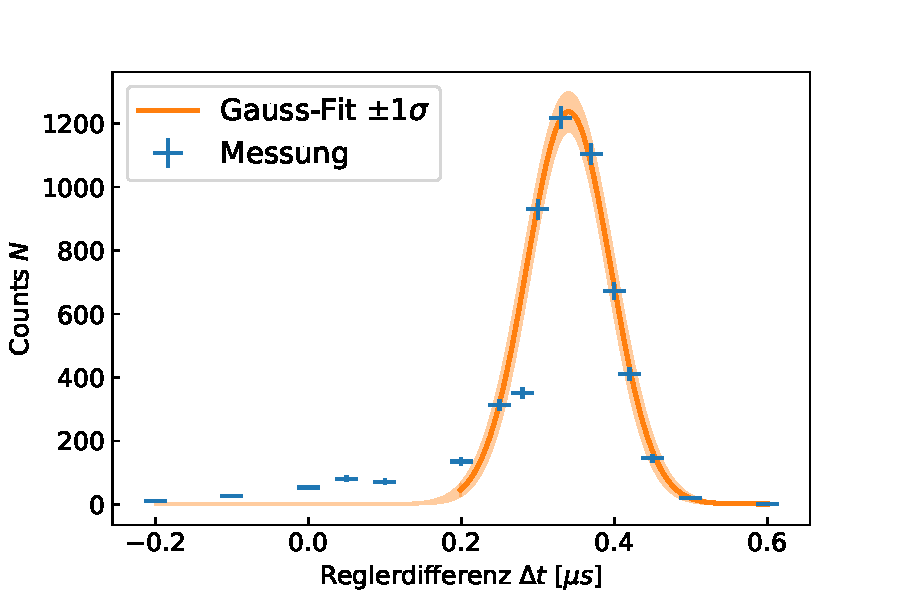
\includegraphics[width=0.7\textwidth]{dat/zeitdifferenz.pdf}
		\caption{Zusammenhang von der eingestellten Verzögerung zwischen beiden Signalen und der Zählrate.
			Die Daten wurden mit einer Gauß-Kurve \\$N(\Delta t) =  A \cdot \exp{-\frac{(\Delta t - \Delta t_0)^2}{2 \sigma_{\Delta t}^2}} + y_0$ angepasst.}
		\label{fig:zeitdiff}
	\end{figure}
	Da Werte mit Verzögerungsdauern kleiner als \SI{0.2}{\micro\second} eine statistisch relevante Abweichung von Null haben, wurden diese nicht in die Anpassung der Gauß-Kurve eingebunden.
	Die Position des Peaks liegt bei $\Delta t_0 = \input{dat/messung1_x0.txt}$.
	In allen folgenden Messungen ist die Signalverzögerung fest auf \SI{333}{\nano\second} eingestellt.
	Diese Einstellung ist mit der Peakposition kompatibel und liefert eine Signaleffizienz von $\epsilon = \input{dat/messung1_eff.txt}$ im Bezug zum Peakmaximum.
	Die Breite $\sigma_{\Delta t} = \input{dat/messung1_d.txt}$ der Kurve ist eine grobe Abschätzung für die Zeitauflösung.
	
\subsection{Koinzidenzauflösungszeit}
	
	Eine genauere Bestimmung der Auflösungszeit $2\theta$ von zwei aufeinander folgenden Signalen ist mit
	\begin{equation}
		N_\text{Z} = N_1 \cdot N_2 \cdot 2\tau \quad \Leftrightarrow \quad  2\tau = \frac{N_Z}{N_1 N_2} = \input{dat/messung2_zweiT.txt}
	\end{equation}
	möglich.
	Dabei sind $N_1 = \input{dat/messung2_det1.txt}$, $N_2 = \input{dat/messung2_det2.txt}$ die Zählraten beider Detektoren vor und $N_Z = \input{dat/messung2_koinz.txt}$ die Zählrate nach der Koinzidenzeinheit.
	Das berechnete Ergebnis liegt in der Größenordnung der Abschätzung.
	Die Quelle hatte im Jahr 1962 eine Aktivität von \SI{3.7}{\mega\becquerel} und somit werden bei der Messung ca. \SI{0.4}{\%} aller Zerfälle gemessen.

	Die Koinzidenzeinheit sieht zwei Signale mit einer absoluten Verzögerung von $\tau$ als Koinzidenz an.
	Somit kann ein Signal relativ zum anderen um maximal $2 \tau$ verschoben werden, ohne aus diesem Interval zu fallen.
	
	Bei dieser Messung wurde $^{137}\text{Cs}$ verwendet, damit ausschließlich einzelne und somit zufällige Koinzidenzen auftreten können.
	
	Durch verschiedene Reflexions- und Streueffekte treten unter bestimmten Winkeln erhöhte Zählraten auf.
	Zum einen werden Photonen bevorzugt bei $\theta = \SI{180}{\degree}$ zurückgestrahlt.
	Zusätzlich werden Photonen durch den Comptoneffekt in der Bleiabschirmung abgelenkt und können bei kleineren Winkeln $\theta$ leicht in den anderen Detektor treffen.
	Bei $\theta = \SI{120}{\degree}$ sind beide Effekte klein und es werden größtenteils die ursprünglichen zufälligen Koinzidenzen der Quelle gemessen.
	Für eine genauere Analyse ist eine tiefere Betrachtung der auftretenden Effekte und der genauen Geometrie des Versuchs erforderlich.
		
\subsection{Vernichtungsstrahung}

	Die $^{22}\text{Na}$-Quelle führt hauptsächlich zur Bildung von Parapositronium, welches dann unter einem Winkel von \SI{180}{\degree} in zwei $\gamma$-Quanten zerfällt.
	In \cref{fig:vernichtung} ist die Zählrate der Koinzidenzen gegen den Winkel $\theta$ dargestellt.
	Dabei wurde die Zählrate an zufälligen Koinzidenzen $N_\text{Z} = \input{dat/messung3_koinz.txt}$ bereits von der gemessenen Zählrate abgezogen, auch wenn sie keinen messbaren Anteil an der Gesamtzählrate hat.
	Theoretisch wird ein scharfer Peak bei genau \SI{180}{\degree} erwartet.
	
	\begin{figure}[ht]
		\centering
		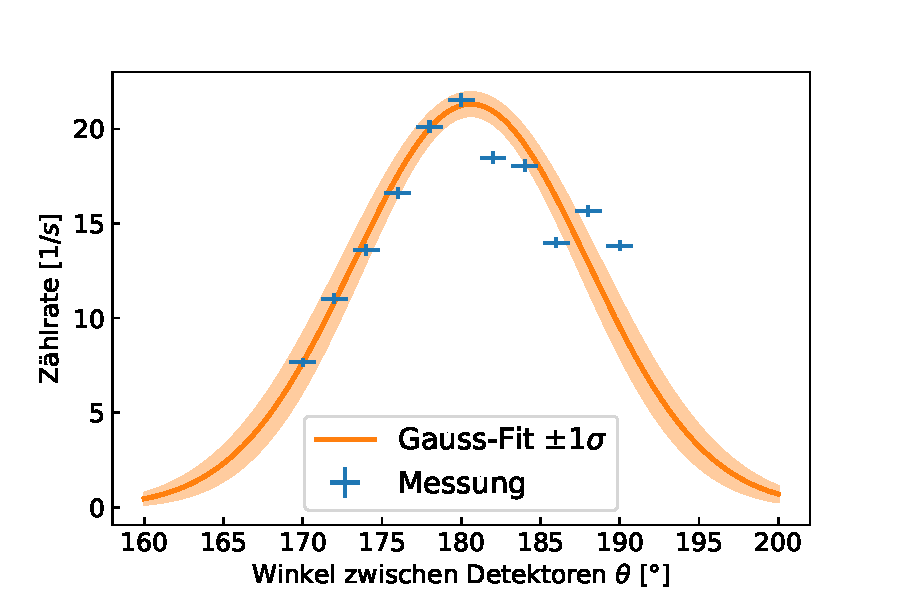
\includegraphics[width=0.7\textwidth]{dat/vernichtung.pdf}
		\caption{Winkelspezifische Zählrate der $^{22}\text{Na}$-Quelle.
			An die Daten wurde eine Gauß-Kurve mit $C(\theta) = A \cdot \exp{-\frac{(\theta - \theta_0)^2}{2 \sigma_{\theta_0}^2}} + y_0$ angepasst.
			Der Peak bei $\theta_0 = \SI{180,6 \pm 0,5}{\degree}$ weißt durch die ausgedehnte Detektorgeometrie eine Breite von $\sigma_{\theta_0} = \SI{7,4 \pm 0,6}{\degree}$ auf.}
		\label{fig:vernichtung}
	\end{figure}

	Wie in der Grafik zu sehen, wird eine gaußförmige Verteilung mit $\theta_0 = \input{dat/messung3_x0.txt}$ und $\sigma_{\theta_0} = \input{dat/messung3_d.txt}$ an die Daten angelegt.
	Daraus ist abzuleiten, dass die Detektorgeometrie einen hohen Einfluss auf die Unsicherheit der betrachteten Winkelmessung hat.
	Im Folgenden ist die Unsicherheit einer Winkelmessung durch $\sigma_{\theta_0}$ gegeben.
	Das $\theta_0$ leicht von \SI{180}{\degree} verschoben ist, kann an einer Schieflage der Quelle während der Messung liegen.
	Da $\theta_0$ allerdings immer noch ausreichend nahe am theoretischen Wert liegt, wurde hier keine weitere Korrektur berechnet.
	
	%TODO fragen beantworten
	
	%TODO mit anteil aus sec2 übereinstimmend?
	%Falls alle Strahlung gemessen wird: 100\% abgedeckter Raumwinkel = 4 pi
	%anteil * 4 pi = 2 pi (1-cos(a / 2))

\subsection{Winkelkorrelation}

	Nachdem aus den vorherigen Messungen Korrekturen und Unsicherheiten des Messapparates bestimmt worden sind, soll nun die Winkelkorrelation der $^{60}\text{Co}$-Probe ermittelt werden.
	Dazu wird zunächst die zufällige Koinzidenzrate zum einen mit der obigen $2\tau$ Methode bestimmt und zum anderen direkt gemessen.
	Die errechnete Koinzidenzrate aus den Einzelraten der Detektoren ergibt $N_\text{Z} = \input{dat/messung4_koinz.txt}$, während die gemessene etwa um den Faktor 10 größer ist.
	Da allerdings insgesamt nur 9 Ereignisse registriert worden sind, können damit keine statistischen Aussagen gemacht werden.
	Sie sind im Verhältnis zur gemessenen Zählrate echter Koinzidenzen verschwindend gering und wirken sich dadurch nicht auf das Ergebnis aus.
	In \cref{fig:theoKurve} sind die Messwerte für $\theta = \SI{90}{\degree}$ und $\theta = \SI{180}{\degree}$ sowie die theoretische Winkelkorrelation eingezeichnet.
	
	\begin{figure}[ht]
		\centering
		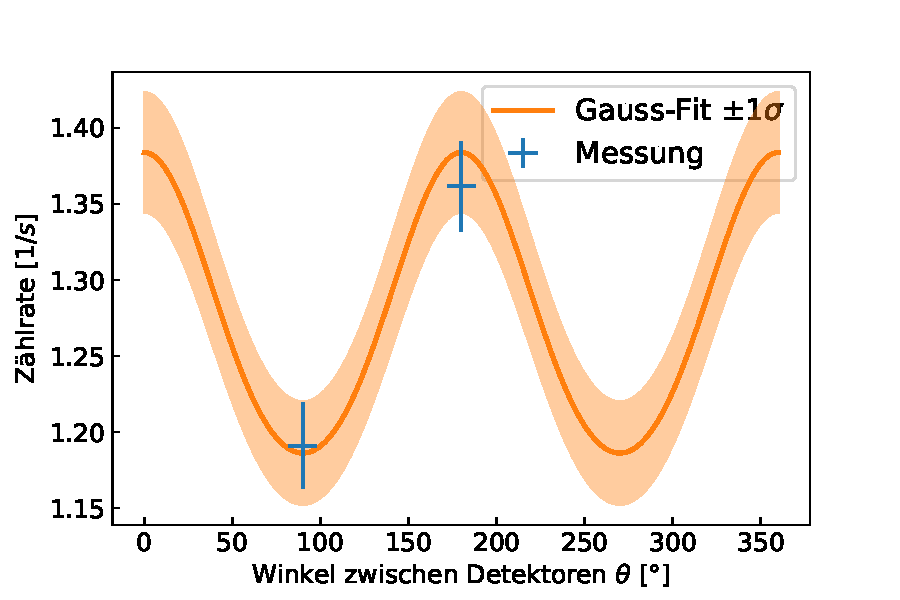
\includegraphics[width=0.7\textwidth]{dat/theoKurve.pdf}
		\caption{Theoretischer Kurvenverlauf und gemessene Einzelwerte.
			Die theoretische Kurve ist proportional zu $1 + \frac{1}{8} \cos^2 \theta + \frac{1}{24} \cos^4 \theta$.}
		\label{fig:theoKurve}
	\end{figure}

	Vergleicht man die theoretische mit der experimentellen Asymmetrie
	\begin{align*}
		A_\text{theo} =&\, \frac{W(\SI{180}{\degree}) - W(\SI{90}{\degree})}{W(\SI{90}{\degree})} = \input{dat/messung4_Atheo.txt} \\
		A_\text{exp} =&\, \frac{C(\SI{180}{\degree}) - C(\SI{90}{\degree})}{C(\SI{90}{\degree})} = \input{dat/messung4_Aexp.txt},
	\end{align*}
	wobei die theoretische Winkelkorrelation $W(\theta)$ aus \cref{eq:korrelation} stammt und $C(\theta)$ die gemessene Zählrate angibt.
	Die gemessene stimmt mit der theoretischen Asymmetrie für die \mbox{$\gamma$-$\gamma$-Kaskade} überein.
	Allerdings ist die Unsicherheit der ermittelten Asymmetrie groß und liegt bei über \SI{20}{\percent}.
	Um die Unsicherheit zu verringern, müssen mehr Messpunkte aufgenommen, die Winkelauflösung verbessert und im Allgemeinen längere Messzeiten eingeplant werden.
	